 In this chapter, we explore the related work of virtualized TAS. We first outline recent 
 works on TCP acceleration (section 3.1), then we list the state-of-the-art methods for network virtualization (section 3.2).



\section{TCP acceleration techniques}


\section{Network Virtualization}
Public cloud providers, such as Amazon Web Services (AWS), Microsoft Azure, 
and Google Cloud Platform (GCP), have taken different approaches to network 
virtualization for their customers. While Microsoft has been following a 
hardware-assisted procedure to provision networking demands, Google has been 
utilizing a software-only approach. Section 3.2.1 elaborates on network 
virtualization using a pure software technique, and section 3.2.2 explores 
hardware-assisted network virtualization.


\subsection{Network Virtualization in Software}
\textbf{OpenFlow} was first proposed to enhance the implementation of 
new protocols on top of the production networks. It proposes a standardized 
interface to add and remove entries to flow tables residing on the Ethernet 
switches.\cite{mckeown2008openflow}

\begin{figure}
\small
\center
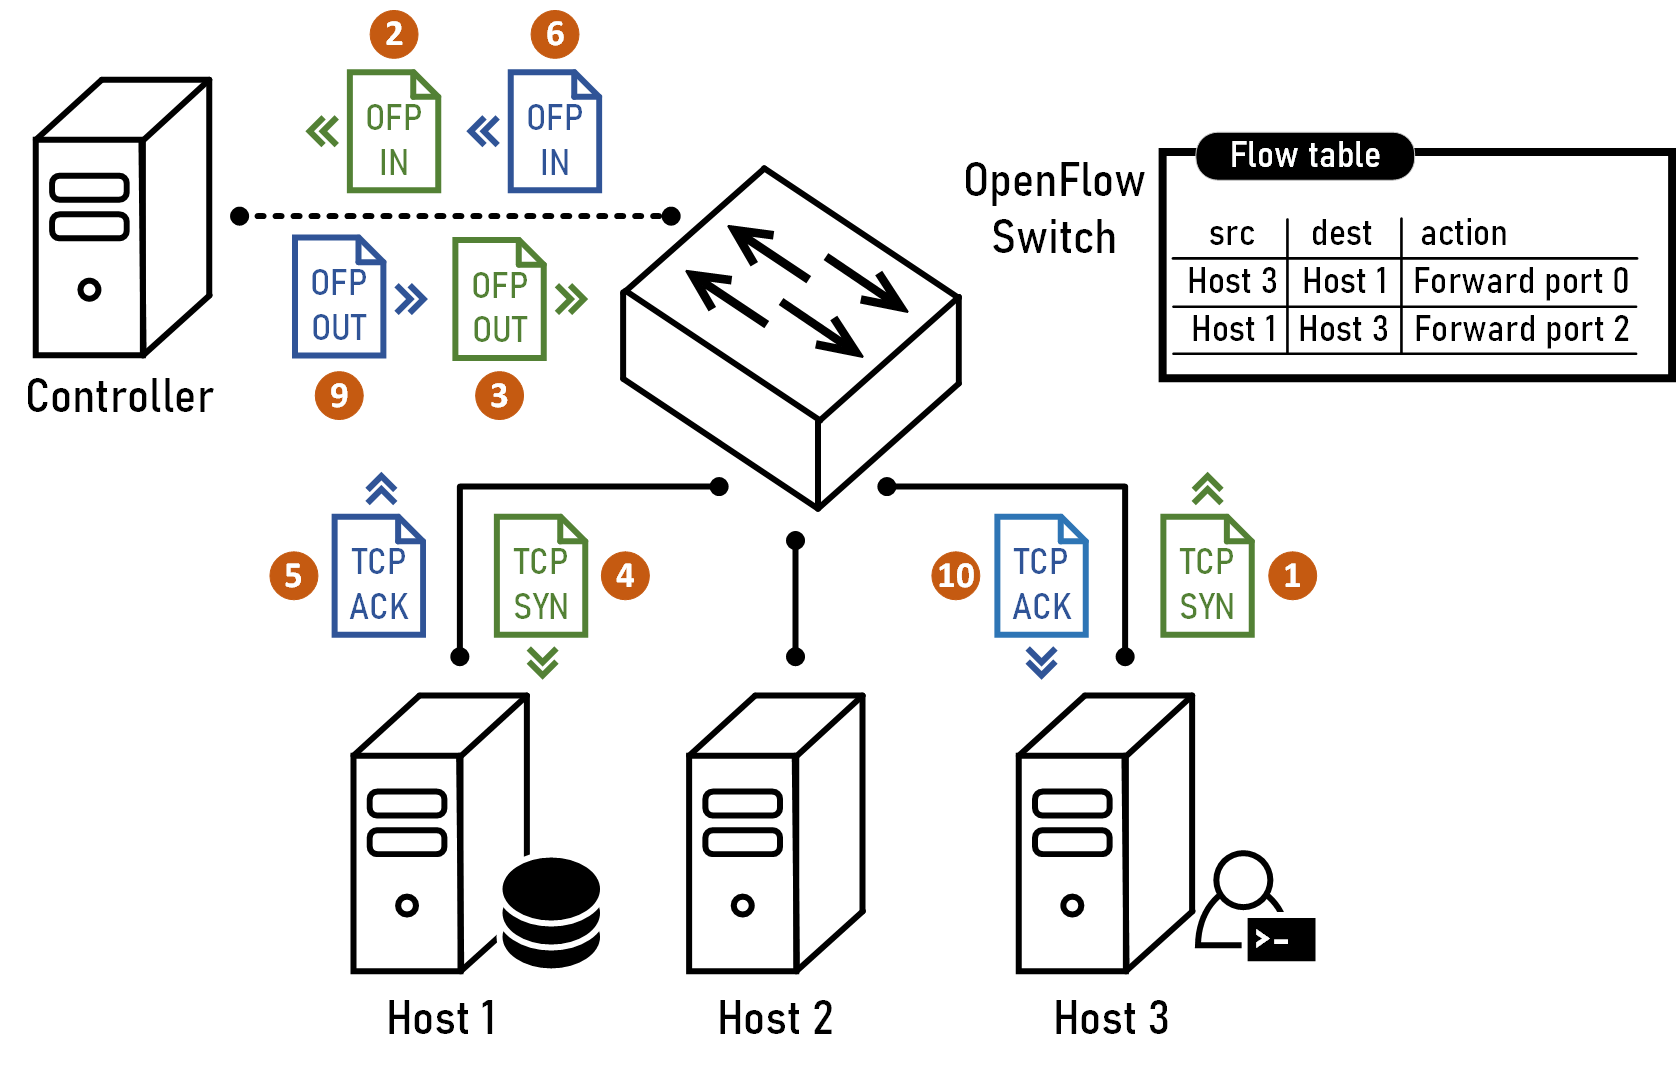
\includegraphics[width=\textwidth]{../Figures/openflow.png}
\caption{OpenFlow}
\label{fig:openflow}
\end{figure}

Open Flow has the following three main components:
\begin{enumerate}
    \item A Flow-table residing on the switch
    \item Secure interface between a controller and the switch
    \item Standardized OpenFlow interface for programming the flow table
\end{enumerate}



In OpenFlow, we can specify packet headers. OpenFlow switch then matches the 
packets with the specified headers and gr
Packets can be matched based on specific headers. For example, all packets from
a particular sender could be specified with the sender's IP address in the header. 

A flow is a set of packets that have similar characteristics. It could be a 
TCP connection, or all packets from a particular IP address, or packets 
with the same VLAN tag. 
% OpenFlow has three main component. 
% 1. Flow-table residing on switch
% 2. Secure interface between controller and the open flow switch
% 3. Standardized OpenFlow interface for programming to program flow-table on the switch


% What is flow? 
% Flow could be a TCP connection, or all packets from a particular IP address,
% or all packets from the same VLAN tag.
% Flow are packets that match a specific header


% What are actions on flows?
% 1. Forward this flow to a given port (or ports) 
% 2. Encapsulate and forward flows's packets to a controller
% 3. Drop the flow's packets. 

\subsection{Network Virtualization using hardware}
